\documentclass[13pt,oneside]{book}
\usepackage[utf8]{inputenc}
\usepackage{url}
\usepackage{listings}
\usepackage{graphicx}

\usepackage{geometry}
\geometry{a4paper, left=20mm, right=20mm, top=20mm, bottom=20mm}
\usepackage[margin=1.2in]{geometry}
\usepackage[toc,page]{appendix}
\usepackage{graphicx}
\usepackage{natbib}
\usepackage{lipsum}
\usepackage{caption}

\begin{document}

\captionsetup[figure]{margin=1.5cm,font=small,labelfont={bf},name={Figure},labelsep=colon,textfont={it}}
\captionsetup[table]{margin=1.5cm,font=small,labelfont={bf},name={Table},labelsep=colon,textfont={it}}
\setlipsumdefault{1}

\begin{titlepage}
\begin{center}
{\LARGE College Of Engineering Trivandrum}\\[3cm]
\linespread{1.2}\huge {\bfseries System Software Lab}\\[3cm]
\linespread{1}

\includegraphics[width=5cm]{img/emblem.jpeg}\\[3cm]
{\Large GOKUL K\\ S5  CSE \\ Roll No:21\\ TVE18CS021 }\\[1cm]


\textit{ }\\[2cm]
Department of Computer Science\\[0.2cm]
\today
\end{center}

\end{titlepage}

\newpage

\begin{frame}{}
    \centering
    \hspace*{-0.5cm}
    $\vcenter{\hbox{
\includegraphics[width=1.5cm]{img/emblem.jpeg}}}$
    $\vcenter{\resizebox{0.95\textwidth}{!}{
        \begin{tabular}{c}
             CS331 - System Software Lab $\cdot$ 2020 $\cdot$   \\
             \hline 
        \end{tabular}
    }}$
\end{frame}
\section*{Cycle 1}
\section*{Expt 2}
\begin{center}
    \Large{Disk Scheduling Algorithms}
\end{center}
\section*{Aim}
\large
Simulate the following disk scheduling algorithms.\\
a) FCFS\\
b)SCAN \\
c) C-SCAN \\

\section*{Algorithm}
    \subsection*{FCFS}
    \begin{verbatim}
        1 Let Request array represents an array storing indexes of tracks
            that have been requested in ascending order of their time of
            arrival head is the position of disk head .
        2 Let us one by one take the tracks in default order and calculate
            the absolute distance of the track from the head .
        3 Increment the total seek count with this distance .
        4 Currently serviced track position now becomes the new head
            position .
        5 Go to step 2 until all tracks in request array have not been
            serviced .
    \end{verbatim}  
    \subsection*{SCAN}
    \begin{verbatim}
        1 Let Request array represents an array storing indexes of tracks
            that have been requested in ascending order of their time of
            arrival . head is the position of disk head .
        2 Let direction represents whether the head is moving towards left
            or right .
        3 In the direction in which head is moving service all tracks one by
            one .
        4 Calculate the absolute distance of the track from the head .
        5 Increment the total seek count with this distance .
        6 Currently serviced track position now becomes the new head
            position .
        7 Go to step 3 until we reach at one of the ends of the disk .
        8 If we reach at the end of the disk reverse the direction and go to
            step 2 until all tracks in request array have not been serviced
    \end{verbatim}
    \subsection*{C-SCAN}
    \begin{verbatim}
        1 Let Request array represents an array storing indexes of tracks
            that have been requested in ascending order of their time of
          arrival head is the position of disk head .
        2 The head services only in the right direction from 0 to size of
            the disk .
        3 While moving in the left direction do not service any of the
            tracks .
        4 When we reach at the beginning ( left end ) reverse the direction .
        5 While moving in right direction it services all tracks one by one .
        6 While moving in right direction calculate the absolute distance of
            the track from the head .
        7 Increment the total seek count with this distance .
        8 Currently serviced track position now becomes the new head
            position .
        9 Go to step 6 until we reach at right end of the disk .
    \end{verbatim}  
    
    \section*{Source Code}
    \Large\textbf{fcfs.c}
\small

\begin{lstlisting}[language=C]
void fcfs(int * pos_arr, int n, int curr_head_pos)
{
	int temp, curr_pos = 0, seek_count = 0;
	size_t i;

	printf("%d -> ", curr_head_pos);
	for(i = 0; i < n; i++)
	{
		temp = pos_arr[i];
		printf("%d", temp);
		if(i != n-1) printf(" -> ");

		seek_count += abs(temp - curr_pos);
		curr_pos = temp;
	}

	printf("\nTotal seek count: %d\n", seek_count);
}
    \end{lstlisting}
    
        \Large\textbf{scan.c}
\small

\begin{lstlisting}[language=C]
void scan(int * pos_arr, int n, int curr_head_pos)
{
	int temp, curr_pos = curr_head_pos, seek_count = 0, direction = 1;
	int i = n-1, j = 0;

	printf("\nSelect initial direction (1 for LTR, -1 for RTL): ");
	scanf("%d", &direction);

	qsort(pos_arr, n, sizeof(int), comp_function);
	
	// Finding the position of head in the sorted array
	while(curr_head_pos > pos_arr[j]) j++;
	temp = (direction == -1) ? j-1: j;

	// Find a better way
	for(i = temp; i >= 0 && i < n; i = i+direction) 
	{
		seek_count += abs(curr_pos - pos_arr[i]);
		curr_pos = pos_arr[i];
		printf("%d -> ", curr_pos);
	}

	seek_count += ((direction == -1)? curr_pos: LIM-curr_pos);
	curr_pos = (direction == -1)? 0: LIM;

	for(i = temp; i >= 0 && i < n; i = i-direction)
	{
		seek_count += abs(curr_pos - pos_arr[i]);
		curr_pos = pos_arr[i];
		printf("%d -> ", curr_pos);
	}

	printf("\nTotal seek count: %d\n", seek_count);
}
    \end{lstlisting}
        \Large\textbf{cscan.c}
\small

\begin{lstlisting}[language=C]
int cscan(int * pos_arr, int n, int curr_head_pos)
{
	int temp, curr_pos = curr_head_pos, seek_count = 0, direction = 1;
	int i = n-1, j = 0;

	printf("\nSelect direction (1 for LTR, -1 for RTL): ");
	scanf("%d", &direction);

	qsort(pos_arr, n, sizeof(int), comp_function);
	
	// Finding the position of head in the sorted array
	while(curr_head_pos > pos_arr[j]) j++;
	temp = (direction == -1) ? j-1: j;

	while(i >= 0)
	{
		printf("%d -> ", pos_arr[temp]);
		seek_count += abs(curr_pos - pos_arr[temp]);
		curr_pos = pos_arr[temp];
		temp = temp+direction;

		if((temp == n && direction == 1) && i != 0)
		{
			printf("%d -> ", LIM);
			temp = 0;
			seek_count += LIM-curr_pos;
			curr_pos = 0;
		}
		else if((temp == 0 && direction == -1) && i != 0)
		{
			printf("%d -> ", 0);
			seek_count += curr_pos;
			curr_pos = n-1;
			temp = n-1;
		}

		--i;
	}

	printf("\nTotal seek count: %d\n", seek_count);
}
    \end{lstlisting}
    \section*{Output}
    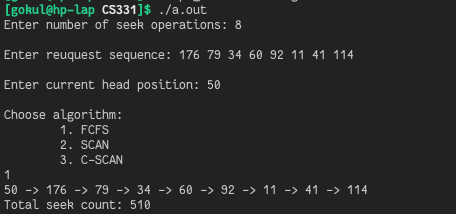
\includegraphics[]{img/p2/ss1.png} \\
    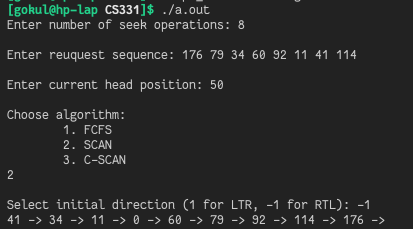
\includegraphics[]{img/p2/ss2.png} \\
    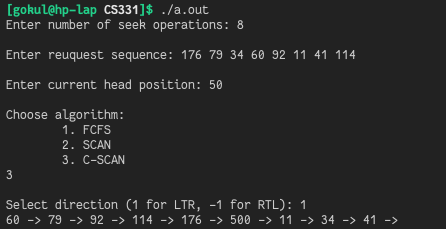
\includegraphics[]{img/p2/ss3.png} 
    
\Large
\section*{Result}
\large
The above algorithms were implemented and its output verified
\end{document}